\chapter{Street Network Grammars}
\section{Shape Grammar} \label{sec:shape_grammar}
The main key of shape grammar is to generate paintings by a new defined grammar based on shapes, selection rules, painting rules and limiting shapes. Shape grammar is a language based on an alphabet of shapes and generated shapes \citep{shapeGrammars:1972}. 

A class of paintings defines the pair (S,M). S represents the shape specifications and M the material specifications. The shape specification contains a shape grammar, defining a language of two dimensional shapes, and a selection rule. M specifies a finite list of material specifications and one limiting shape on a canvas.

\subsection{Shape Grammar Definition}
\label{sec:Shape_Grammar_Definition}
Shape Grammar is defined over an alphabet of shapes and generated n-dimensional shapes \citep{shapeGrammars:1972}.
\begin{displayquote} 
    Definition. A shape grammar (SG) is a 4-tuple: $SG = (V_T, V_M, R, I)$ where
    \begin{enumerate}
        \item $V_T$ is a finite set of shapes.
        \item $V_M$ is a finite set of shapes such that $V_T $* $\cap$  $V_M = \emptyset$
        \item R is a finite set of ordered pairs (u,v) where:
        \begin{enumerate}
         \item u is a shape consisting of an element of $V_T $* combined with an element of $V_M$ \item v is a shape consisting of (A) the element of $V_T $* contained in u or (B) the element of $V_T $* contained in u combined with an element of $V_M$ or (C) the element of $V_T $* contained in u with an additional element of $V_T$* and an element of $V_M$.
        \end{enumerate}
        \item I is a shape consisting of elements of $V_T $* and $V_M$.
    \end{enumerate}
\end{displayquote}

\subsection{Selection Rules}
\label{sec:Shape_Grammar_Selection_Rules}
A painting is generated based on an undefined count of shape rules. This requires a mechanism to select a correct shape. The depth is defined by levels which are being assigned during generation based on their rules: \citep{shapeGrammars:1972}.
\begin{displayquote}
    \begin{enumerate}
        \item The terminals in the initial shape are assigned to level 0.
        \item If a shape rule is applied, and the highest level assigned to any part ot the terminal corresponding to the level side of the rule is N, then
        \begin{enumerate}
            \item if the rule is of type A, any part of the terminal enclosed by the marker in the left side of the rule is assigned to N.
            \item if the rule is of type B, any part of the terminal enclosed by the marker in the left side of the rule is assigned to N and any part of the terminal enclosed by the marker is assigned to N+1.
            \item if the rule is of type C, the terminal added is assigned to N+1.
        \end{enumerate}
        \item No other level assignments are made.
    \end{enumerate}
\end{displayquote}

\subsection{Painting Rules}
\label{sec:Shape_Grammar_Painting_Rules}
Painting rules describe witch shape should be painted inside of a defined area. Like in a Venn diagram the rules contain multiple levels 0 - n. By combining these levels the painting colour is described\citep{shapeGrammars:1972}.
\begin{displayquote}
    A painting rule has two sides separated by a double arrow ($\Rightarrow$). The left side of a painting rule defines a set using the sets determined by level assignment and the usual set operators, for example, union($\bigcap$), intersection ($\bigcup$), complementation($\sim$), and exclusive or ($\bigotimes$). The sets defined by the left side of the painting rules of M must partition the universal set. The right side of a painting rule is a rectangle painted in the manner the set defined by the left side of the rule is to be painted.
\end{displayquote}

\subsection{Limiting Shapes}
\label{sec:Shape_Grammar_Limiting_Shapes}
These shapes define a limiting area on the canvas, where shape painting is allowed. 
The area could have any form, but normally it is defined as a rectangle. Like a camera view the limiting shape defines the scale of a painting and its viewpoint. Therefore the initial/start shape could be outside of the limiting shape.

\subsection{Example\citep{shapeGrammars:1972}}
\subsubsection{Shape Grammar}
\begin{align}
\label{eq:Shape_Grammar}
SG1 &= <V_T, V_M, R, I>  \\
\label{eq:Shape_Grammar_VT}
V_T &= \{-\}  \\
\label{eq:Shape_Grammar_VM}
V_M &= \{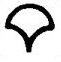
\includegraphics{sg_specification_VM.jpg} \}\ \\
\label{eq:Shape_Grammar_R}
R &= Rules\ [R]\ \ \ \ 
R1=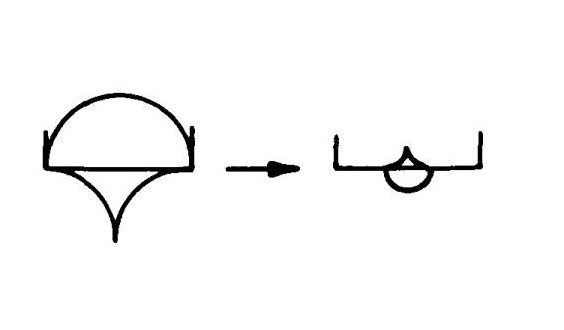
\includegraphics[width=2cm]{sg_specification_rule1.jpg}
R2=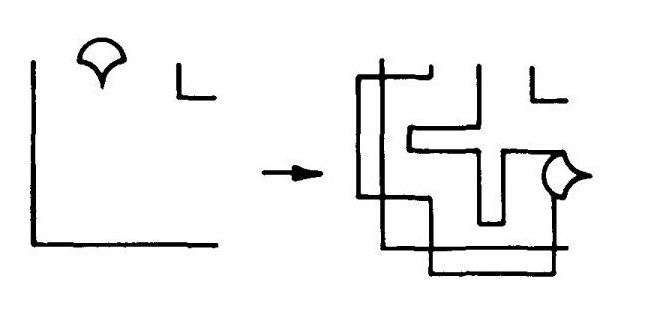
\includegraphics[width=2cm]{sg_specification_rule2.jpg}
R3=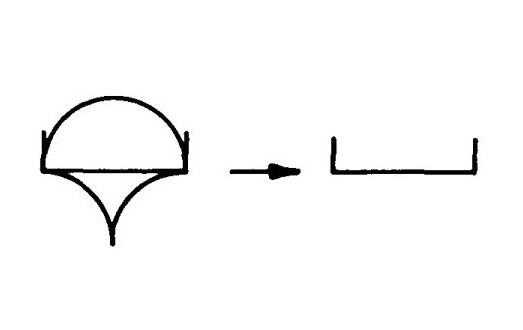
\includegraphics[width=2cm]{sg_specification_rule3.jpg}
\\
\label{eq:Shape_Grammar_I}
I &= Initial\ shape\ I\ \ 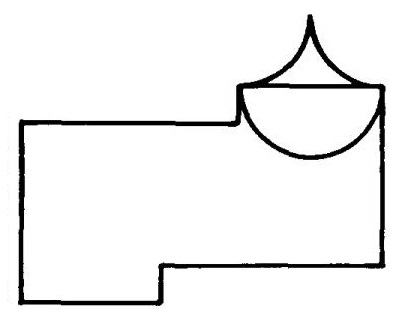
\includegraphics[width=1.5cm]{sg_specification_I.jpg}
\end{align}
\subsubsection{Selection Rule}
\begin{equation}
<0,2>
\end{equation}

\subsubsection{Painting Rules}
\begin{align}
    \label{fig:Shape Grammars/Shape Specification/Painting_Rule_1}
    L0\cap L1\cap L2 \Longrightarrow  
    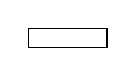
\begin{tikzpicture}
        \filldraw[fill=black!00!white, draw=black] (0,0) rectangle (1,0.25);
    \end{tikzpicture} \\
    \label{fig:Shape Grammars/Shape Specification/Painting_Rule_2}
    (L0\cap L1\cap \sim L2)\cup (L0\cap \sim L1\cap L2)\cup (\sim L0\cap L1 \cap L2) \Longrightarrow  
    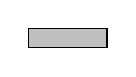
\begin{tikzpicture}
        \filldraw[fill=black!25!white, draw=black] (0,0) rectangle (1,0.25);
    \end{tikzpicture} \\
    \label{fig:Shape Grammars/Shape Specification/Painting_Rule_3}
    (L0\cap \sim L1\cap \sim L2)\cup (\sim L0\cap L1\cap \sim l2)\cup (\sim L0\cap \sim L1 \cap L2) \Longrightarrow  
    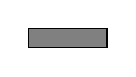
\begin{tikzpicture}
        \filldraw[fill=black!50!white, draw=black] (0,0) rectangle (1,0.25);
    \end{tikzpicture} \\
    \label{fig:Shape Grammars/Shape Specification/Painting_Rule_4}
    \sim (L0\cup L1\cup L2)  \Longrightarrow  
    
\begin{tikzpicture}
        \filldraw[fill=black!100!white, draw=black] (0,0) rectangle (1,0.25);
    \end{tikzpicture}
\end{align}
\subsubsection{Limiting Shape}
\begin{figure}[!h]
    \centering
    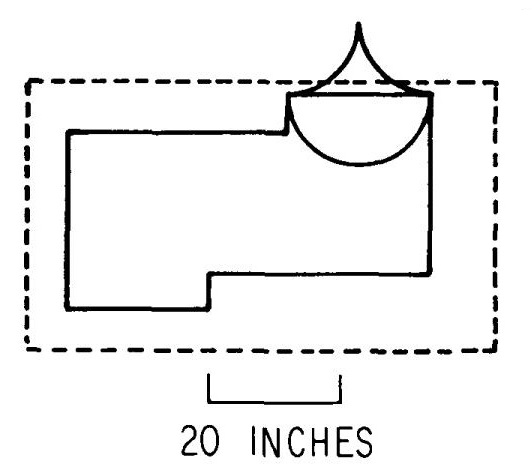
\includegraphics[width=2cm]{sg_specification_Limiting_shape.jpg}
    \caption{ Limiting shape I \citep{shapeGrammars:1972}}\label{fig:Shape Grammars/Shape Specification/Limiting_Shape}
\end{figure}
\pagebreak
\subsubsection{Generated}
The following image \ref{fig:Shape Grammars/Example} shows the generated painting with the relevant steps. The levels are generated as described above \ref{sec:Shape_Grammar_Selection_Rules} 
\newline
Level 0: Steps 0 to 2,\newline Level 1: Steps 3 and 4,\newline Level 2: Steps 18 and 19
\begin{figure}[!h]
    \centering
    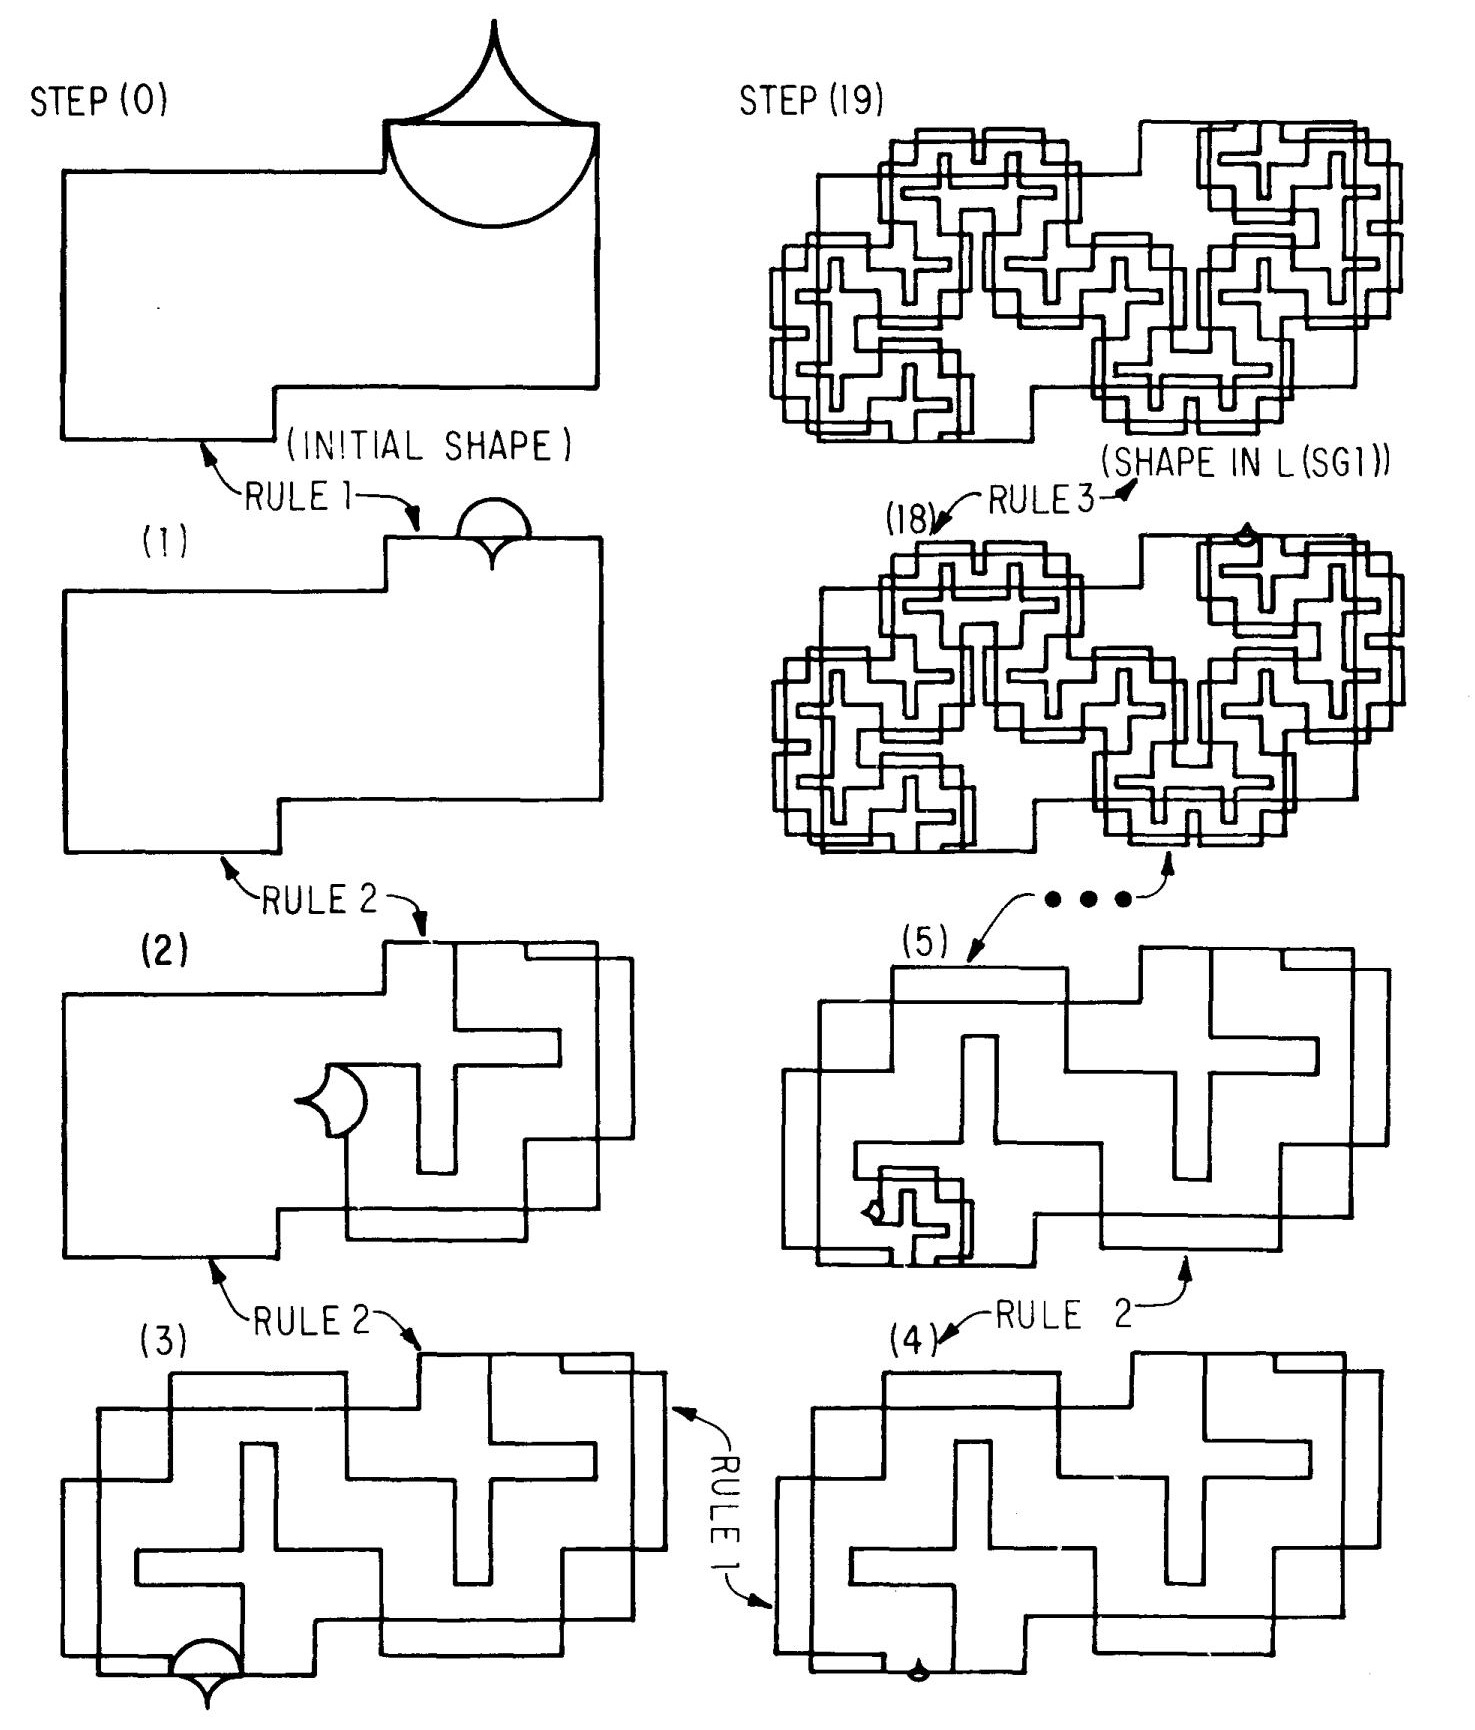
\includegraphics{sg_example.jpg}
    \caption{ Generated Painting\citep{shapeGrammars:1972}}\label{fig:Shape Grammars/Example}
\end{figure}

\pagebreak
\subsection{Street Generation}
In the following section we debate the usefulness of generating street networks by shape grammar. 
\paragraph{Features}
    \begin{itemize}
        \item Can describe and generate veneer in high details.
        \item With R-Shapes windows and high detail 3D-Models can be generated easily.
    \end{itemize}

\paragraph{Problems}
    \begin{itemize}
        \item The given methods generate monotonous streets in most cases. 
        \item A huge number of R-Shapes is required to generate a useful street network.
        \item Areas with different characteristics (historic district, rectangular raster like New York or radial to center like Paris) are difficult to generate.
        \item The R-Rules for the transitions between area characteristics should not repeat themselves and are for that reason difficult to build.
    \end{itemize}

\pagebreak
\section{L-Systems} \label{sec:L-Systems}
L-System is a well established modelling approach for the synthesis of realistic plant images. There are many papers describing L-Systems and how they are applied to generate plant life: "In these cases L-System productions capture the \textit{development} of plant components over time." \citep{PrusinkiewiczEtAl:2001} Productions are applied in parallel, so that all plant parts grow and age equally. The growth is stopped at a defined terminal age. This age is the number of iterations, where in each iteration productions are applied.

The context-free productions in \citep{PrusinkiewiczEtAl:2001} are defined using the following syntax.
\begin{equation} \label{eq:lsystem context free}
    pred : \{block1\}\ cond\ \{block2\} \leadsto succ
\end{equation}
The symbol \textit{pred} (predecessor) defines the module that will get replaced by the modules defined in \textit{succ} (successor). This replacement is only applied, if the (optional) condition is met. \textit{block1} and \textit{block2} are C statement blocks, of which the first block is executed before and the second after the condition is evaluated. \citep{PrusinkiewiczEtAl:2001} gives the following example.
\begin{equation} \label{eq:lsystem example 1}
    A(x) : \{y = x + 2;\}\ y \geq 5\ \{z = y / 3;\}\ \leadsto B(z)C(z + 1)
\end{equation}
If this example production was applied to the module $A(4)$, it would result in the modules $B(2)C(3)$.

The modelling language, described in \citep{PrusinkiewiczEtAl:2001}, also supports context-sensitive productions. The following listing defines the syntax of such a production.
\begin{equation} \label{eq:lsystem context sensitive}
    lcont < pred > rcont : \{block1\}\ cond\ \{block2\} \leadsto succ
\end{equation}
\textit{lcont} (left context) and \textit{rcont} (right context) each define a list of modules that have to precede or respectively follow the \textit{pred} (module being replaced). Context modules are limited to query symbols, which are explained later on. \citep{PrusinkiewiczEtAl:2001} gives the following example.
\begin{equation} \label{eq:lsystem example 2}
    A(x) < B(y) > C(z) : x + z > 0 \leadsto M(y / 2)N(y / 2)
\end{equation}
If the example of listing \ref{eq:lsystem example 2} was applied to the module composition $A(2)B(4)C(0)$, it would result in the modules $A(2)M(2)N(2)C(0)$.

A way to generate images with L-Systems is to use a LOGO-style turtle as a graphical model. Certain modules of the L-System are interpreted as commands to this turtle.

\pagebreak
\section{Space Syntax} \label{sec:space_syntax}
The grammar Space Syntax was first introduced in 1976 by B. Hiller, A. Leaman, P. Stansall and M. Bedford in the paper "Space syntax" \citep{spaceSyntax:1976}. The grammar is based on a morphic language and describes methods to analyse and generate urban areas and buildings.
The language consists of a surface (carrier space) and an ongoing production process of new and different neighbouring parts. Extended Syntax is used to describe special area patterns like ring spaces and block spaces.

The grammar was later extended and integrated into Geographic Information System (GIS). This information system are used to plan and analyse the human interaction with the environment like pedestrian modelling or criminal mapping.
Bin Jiang and Christope Claramunt \citep{integrationSpaceSyntaxGIS:2002} showed the limitation of axial lined-based space syntax (\citep{integrationSpaceSyntaxGIS:2002} chapter: 2.2). They then created a graph representation (\citep{integrationSpaceSyntaxGIS:2002} chapter: 3) and showed that it was at least equivalent to the predefined syntax created by B. Hiller et al.\citep{spaceSyntax:1976}.

Many projects have been developed based on the space syntax graph representation.
